\documentclass[uplatex, dvipdfmx, a4j,11pt]{jsarticle}
\usepackage[dvipdfmx]{graphicx}
\usepackage{lastpage}
\usepackage{fancyhdr}
\usepackage{listings}
\usepackage{jlisting}
\usepackage{xcolor}

\makeatletter
\title{演習課題2}
\author{202310330 長田悠生}
\date{2024年4月28日}

\pagestyle{fancy}

\lstset{
    basicstyle = {\ttfamily}, % 基本的なフォントスタイル
    frame = {tbrl}, % 枠線の枠線。t: top, b: bottom, r: right, l: left
    breaklines = true, % 長い行の改行
    numbers = none, % 行番号の表示。left, right, none
    % stepnumber=1, % 行番号増分
    % numbersep=10pt, % 行番号と本文の間隔 デフォルト:10pt
    showspaces = false, % スペースの表示
    showstringspaces = false, % 文字列中のスペースの表示
    showtabs = false, % タブの表示
    keywordstyle = \color{blue}, % キーワードのスタイル。intやwhileなど
    commentstyle = {\color[HTML]{1AB91A}}, % コメントのスタイル
    identifierstyle = \color{black}, % 識別子のスタイル 関数名や変数名
    stringstyle = \color{brown}, % 文字列のスタイル
    captionpos = t % キャプションの位置 t: 上、b: 下
}

\lstdefinelanguage{Julia}
{
  keywordsprefix=\@,
  morekeywords={
    exit,whos,edit,load,is,isa,isequal,typeof,tuple,ntuple,uid,hash,finalizer,convert,promote,
    subtype,typemin,typemax,realmin,realmax,sizeof,eps,promote_type,method_exists,applicable,
    invoke,dlopen,dlsym,system,error,throw,assert,new,Inf,Nan,pi,im,begin,while,for,in,return,
    break,continue,macro,quote,let,if,elseif,else,try,catch,end,bitstype,ccall,do,using,module,
    import,export,importall,baremodule,immutable,local,global,const,Bool,Int,Int8,Int16,Int32,
    Int64,Uint,Uint8,Uint16,Uint32,Uint64,Float32,Float64,Complex64,Complex128,Any,Nothing,None,
    function,type,typealias,abstract
  },
  sensitive=true,
  morecomment=[l]{\#},
  morestring=[b]',
  morestring=[b]"
}
\renewcommand{\lstlistingname}{}

% headers & footers
\lhead{数値計算法 \@title 提出日:\@date\\\@author}
\chead{}
\rhead{}
\lfoot{}
\cfoot{\thepage/\pageref{LastPage}}
\rfoot{}
\renewcommand{\headrulewidth}{0pt}
\renewcommand{\footrulewidth}{0pt}
\makeatother

\begin{document}
\section*{課題1}
\subsection*{(1-1)}
%\subsubsection*{(1-1)}
\begin{lstlisting}[title={(1-1)のソースコード}, label=code:in, language=Julia]
module report1_1
    using Random
    Random.seed!(0)
    function MonteCarlo(n::Int64)
        if n <= 0
            throw("n have to larger than 0.")
        end
        x::Vector{Float64} = zeros(Float64, n)
        y::Vector{Float64} = zeros(Float64, n)
        for i::Int64 = 1:n
            x[i] = rand()
            y[i] = rand()
        end
        r::Vector{Float64} = zeros(Float64, n)
        for i::Int64 = 1:n
            r[i] = x[i]^2 + y[i]^2
        end
        m::Int64 = 0
        for i::Int64 = 1:n
            if r[i] <= 1
                m = m + 1
            end
        end
        p::Float64 = 4*m/n
        return p
    end
end
\end{lstlisting}

\newpage
\textmc{前ページの関数について具体的なnの値を入れてみたときのソースコードと出力結果です。前ページのソースコードと以下のソースコードは同一のファイルに書いています。}

\begin{lstlisting}[title={上記の関数に具体的なnの値を入れてみたときのソースコード}, label=code:in, language=Julia]
using .report1_1

p_1::Float64 = report1_1.MonteCarlo(1)
println("p_1 = $p_1")

p_100::Float64 = report1_1.MonteCarlo(100)
println("p_100 = $p_100")

p_0::Float64 = report1_1.MonteCarlo(0)
println("p_0 = $p_0")

\end{lstlisting}

\begin{lstlisting}[title={実行結果}, label=code:in, language=sh]
  p_1 = 4.0
  p_100 = 3.28
  ERROR: LoadError: "n have to larger than 0."
  Stacktrace:
   [1] MonteCarlo(n::Int64)
     @ Main.report1_1 C:\Users\admin\Documents\work-space\Julia\numeric-calculation\class2_report\src\report1-1.jl:9
   [2] top-level scope
     @ C:\Users\admin\Documents\work-space\Julia\numeric-calculation\class2_report\src\report1-1.jl:48
  in expression starting at C:\Users\admin\Documents\work-space\Julia\numeric-calculation\class2_report\src\report1-1.jl:48

\end{lstlisting}

\newpage
\subsection*{(1-2)}
\begin{lstlisting}[title={(1-2)のソースコード}, label=code:in, language=Julia]
module monte_carlo
    using Random
    Random.seed!(0)
    function MonteCarlo(n::Int64)
        x::Vector{Float64} = zeros(Float64, n)
        y::Vector{Float64} = zeros(Float64, n)
        for i::Int64 = 1:n
            x[i] = rand()
            y[i] = rand()
        end
        r::Vector{Float64} = zeros(Float64, n)
        for i::Int64 = 1:n
            r[i] = x[i]^2 + y[i]^2
        end
        m::Int64 = 0
        for i::Int64 = 1:n
            if r[i] <= 1
                m = m + 1
            end
        end
        p::Float64 = 4*m/n
        return p
    end

    function MonteCarloData(size::Int64)
        n_vec::Vector{Int64} = zeros(Int64, size)
        result_vec::Vector{Float64} = zeros(Float64, size)
        for i::Int64 = range(1, size, size)
            n::Int64 = 10^i
            result::Float64 = MonteCarlo(n)
            n_vec[i] = n
            result_vec[i] = abs(result - pi)
        end
        return n_vec, result_vec
    end
end

using .monte_carlo
using Plots

n_vec::Vector{Int64}, result_vec::Vector{Float64} = monte_carlo.MonteCarloData(6)

plot(n_vec, result_vec, xaxis=:log)

savefig("report1-2.png")

\end{lstlisting}

\begin{figure}[h]
  \begin{center}
    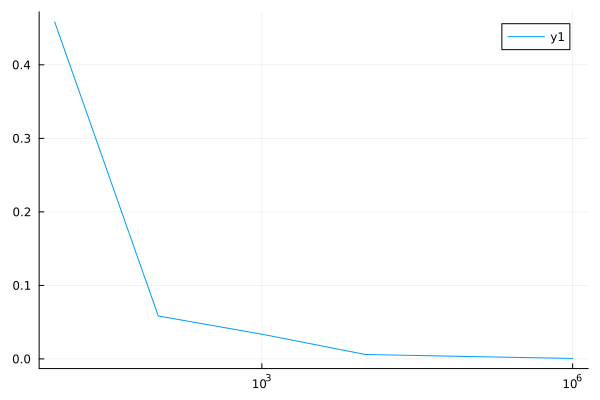
\includegraphics[width=78mm]{report1-2.png}
    \caption{実行結果のグラフ}
  \end{center}
\end{figure}

\section*{課題2}
\subsection*{(2-1)}

\end{document}
